\documentclass[letterpaper,11pt]{article}

\usepackage[open,openlevel=1]{bookmark}
\usepackage{amsmath}
\usepackage{graphicx}
\usepackage[ruled,vlined]{algorithm2e}
\usepackage{mcode}
\usepackage{subcaption}

\begin{document}

\title{Project 1: Fractal Geometry \\ 
		\large MAT128B Winter 2020}
\author{Caitlin Brown, Nikos Trembois, and Shuai Zhi}
\date{February 19, 2020}
\maketitle
\tableofcontents
\newpage

\section*{Introduction}
In this project, numerical analysis is used to understand and demonstrate fractals and their characteristics. The fractals will be generated from the orbits of complex functions. Orbits are the sequence of numbers that results picking a seed value as a function input, then the outputs are introduced as inputs and so on ad infinitum. So $orb(z_0) = z_0, z_1 = \phi(z_0), z_2 \phi(\phi(z_0)) ...$ is the orbit of the initial point $z_0$ under the function $\phi$. This clearly results in an iterative process, thus computers facilitate the generation of orbits. It is not hard to imagine that for certain initial values this process will diverge while other initial values will converge, or at least remain bounded by some value. The filled Julia set is all points whose orbit, using a polynomial function, remains bounded. The boundary of the filled set is called the Julia set.

The Mandelbrot set is defined as the set of complex numbers c for which the sequence c, $c^2 +c$, $(c^2 + c)^2 +c$,... does not tend to infinity as the number of iterations tends to infinity. The Mandelbrot set appears to contain smaller copies of itself, however it is actually not self-similar. Each mini-Mandelbrot set has its own unique patterns.

In this project, fractals, specifically Julia and Mandelbrot sets, are explored. It is easy to get lost in their hypnotizing shapes, but one should not forget their utility in practice which is demonstrated with an application to Newton's method on the complex plane. 

\section{Unit Disk}
The orbit of complex values whose real and imaginary part were within [-1, 1] were calculated for the function $\phi(z) = z^2$. The filled Julia set is the map of the complex plane to its orbit under some function. The filled Julia set under $\phi(z) = z^2$ is the unit disk and is shown in figure \ref{fig:unitDisk}. Under the same function the Julia set would create the unit circle, as it is the boundary of the filled Julia set. It is not surprising that the orbit of $z^2$ should be the unit disk. The square of values less than 1 in magnitude is a value less than the original value (i.e. $x^2 < x$ if $x < 1$), so if the square is applied over and over to the result, it will approach zero and be bounded. Conversely, if a value is greater than 1 the square of the value is greater than the initial value, thus continually applying the square to the result will lead to values that grow unbounded. However, for other functions the outcome is not as intuitive. The algorithm for this problem is shown in Part 1 of the code and the function it calls can be found at the end of the code. Since most problems use a similar iteration in some form a function was created with a few options to do the calculations for multiple parts. The algorithm creates an array of points in the cartesian plane then inputs those points into a function. Then it determines if the value has grown too much to be considered bounded, which the user can set the maximum value for. If it has it either gives that point in the cartesian plane a discrete value or the value of the number of iterations it took to diverge.

\begin{figure}
	\centering
	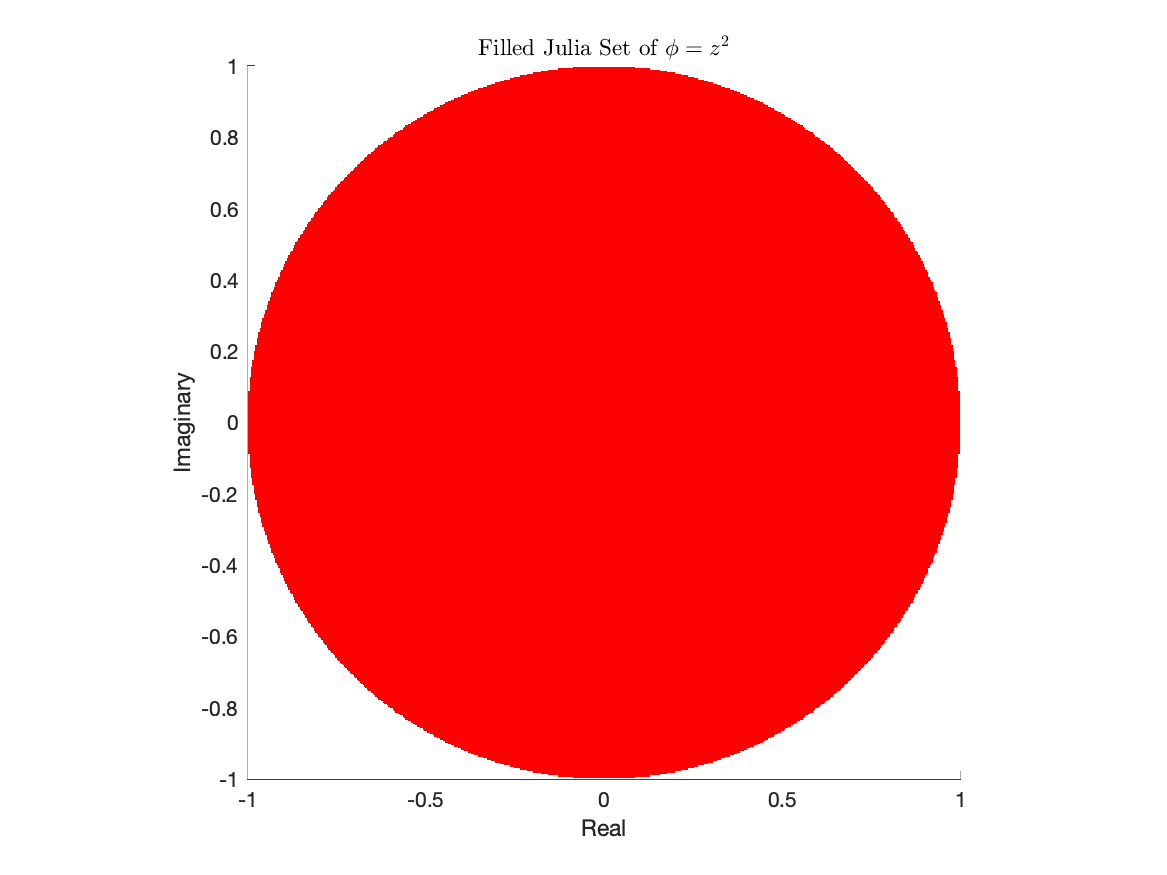
\includegraphics[width=3.5in]{../Figures/UnitDisk.png}
	\caption{Orbit of $z = a + bi$ for $a = b = [-1,1]$ under $\phi=z^2$}
	\label{fig:unitDisk}
\end{figure}

\section{Introduction to Fractals}
The unit disk is a great illustration of the orbit of different initial points under $\phi=z^2$. However, adding a constant to the function (i.e. $\phi(z) = z^2 + c$) creates more interesting maps, which turn out to be fractals. 

\begin{figure}
\centering
	\begin{subfigure}[b]{0.49\linewidth}
		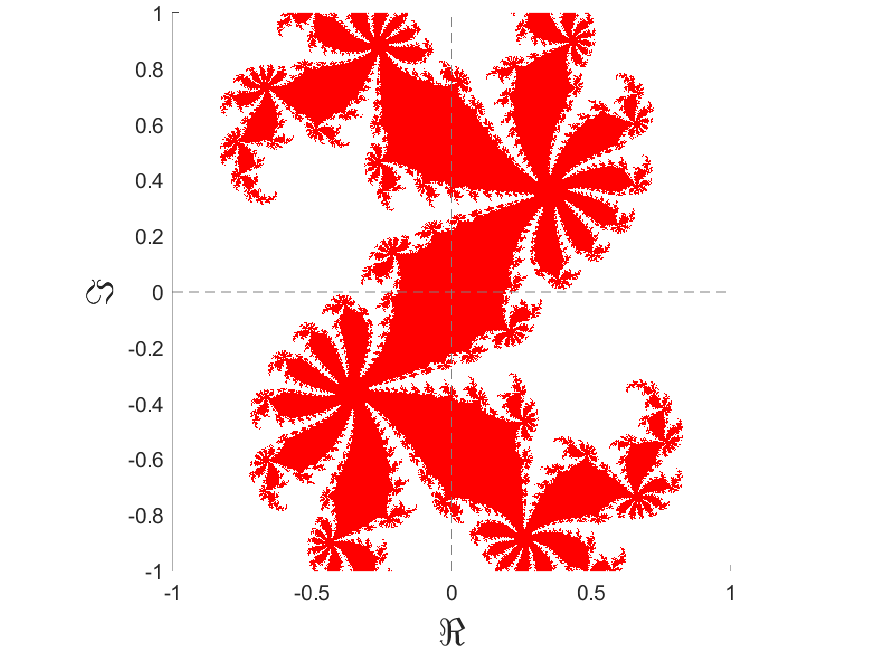
\includegraphics[width=\linewidth]{../Figures/FilledJulia1.png}
		\caption{Filled Julia Set of $z = 0.36 + 0.1i$}
		\label{fig:FJ+.36+.1i}
	\end{subfigure}
	\begin{subfigure}[b]{0.49\linewidth}
		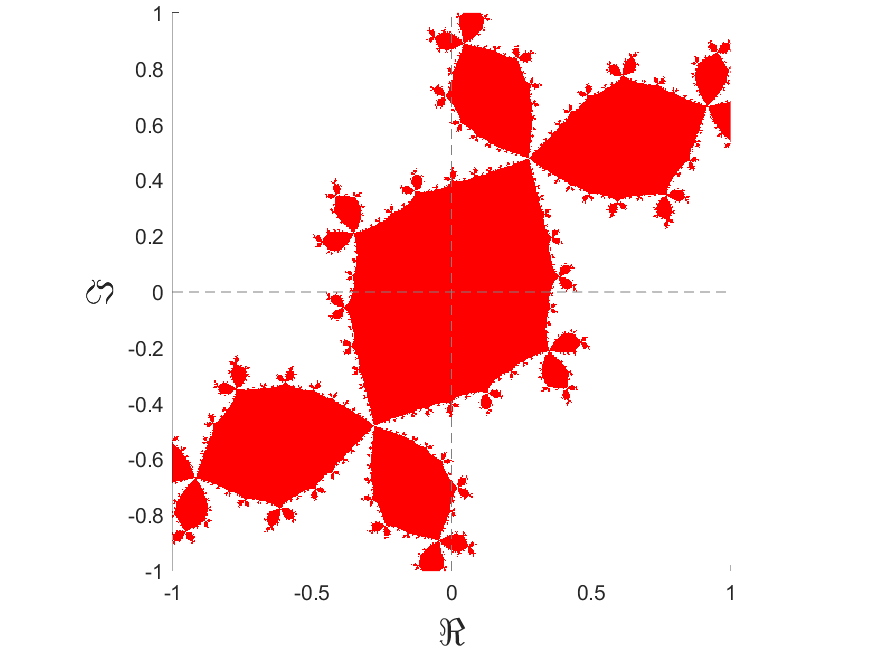
\includegraphics[width=\linewidth]{../Figures/FilledJulia2.png}
		\caption{Filled Julia Set of $z = -0.123 + 0.745i$}
		\label{fig:FJ+.123+.745i}
	\end{subfigure}
	
	\vskip\baselineskip
	
	\begin{subfigure}[b]{0.49\textwidth}
		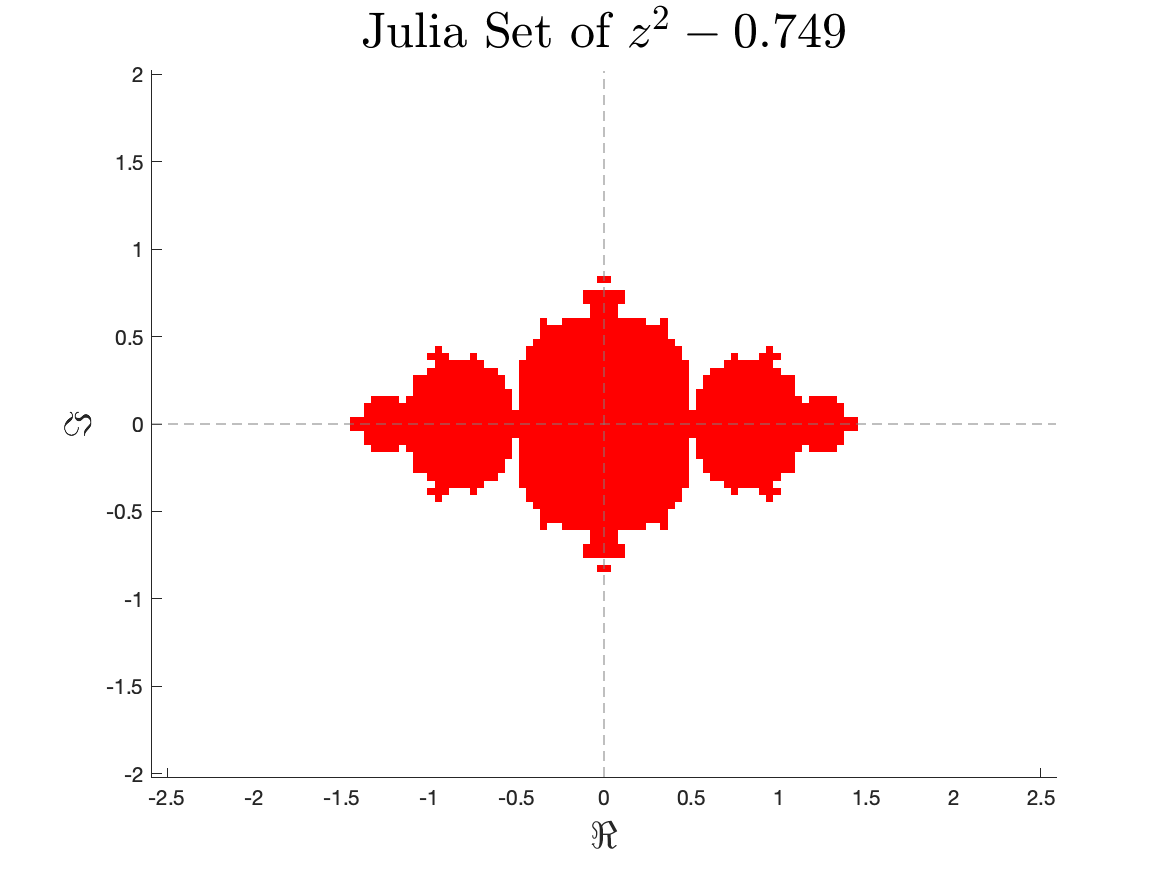
\includegraphics[width=\textwidth]{../Figures/FilledJulia3.png}
		\caption{Filled Julia Set of $z = - 0.749$}
		\label{fig:FJ-.749}
	\end{subfigure}
	\begin{subfigure}[b]{0.49\textwidth}
		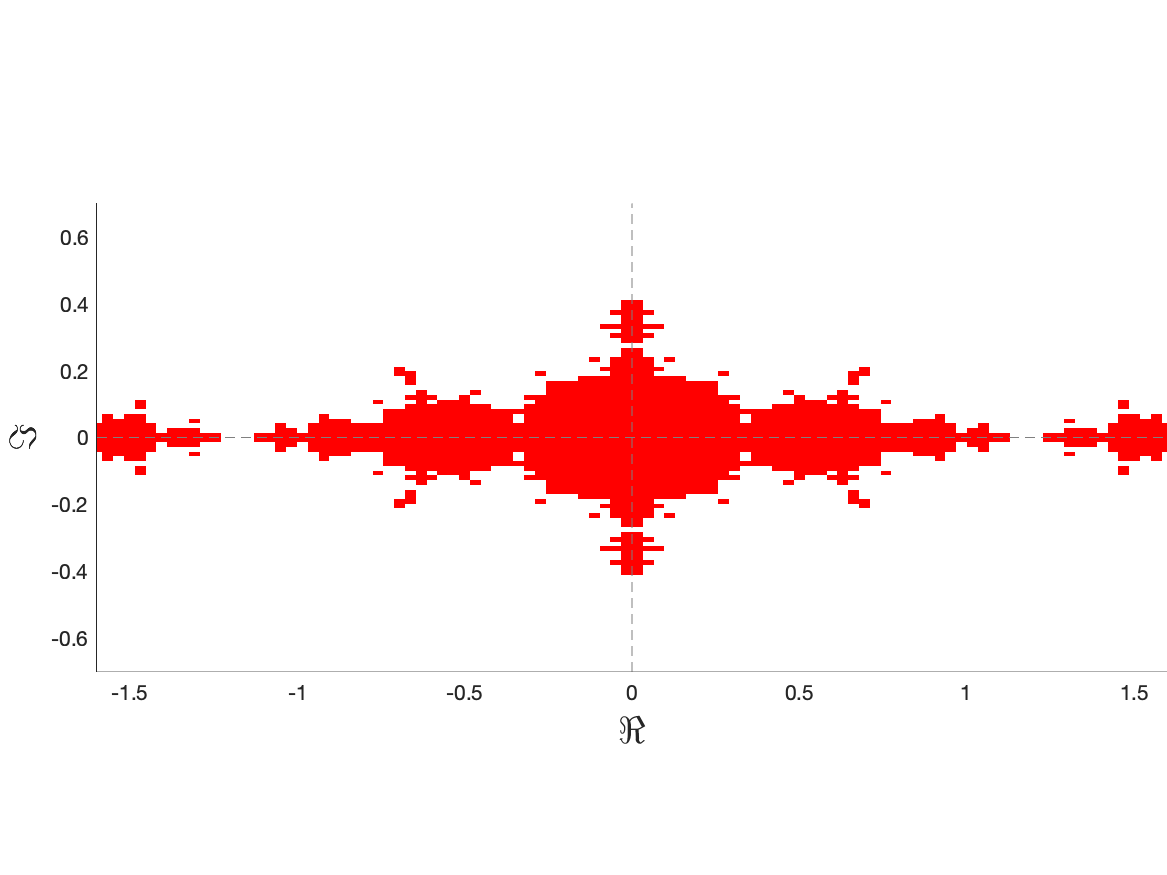
\includegraphics[width=\textwidth]{../Figures/FilledJulia4.png}
		\caption{Filled Julia Set of $z = -1.25$}
		\label{fig:FJ-1.25}
	\end{subfigure}
	\caption{Filled Julia sets with 500 points in real and imaginary axis}
	\label{fig:FJwithC}
\end{figure}

\section{Julia Set}
The Julia set is the boundary of the filled Julia set. So, it marks the edge of the points whose orbits converge under a given function. All points inside the boundary converge, including the line, while those outside of it diverge. The Julia set is found using the inverse iteration method, which is an attractor. As the name suggests, initial points will be attracted to certain values as it is iterated. In fact, the plots below are examples of a specific type of attractor called strange attractors. This is because the attractor maps to a fractal shape. Since the Julia set uses inverse function, $\phi = z^2 + c$ becomes  $\psi = \sqrt{z - c}$. Due to the square root, any given iteration is actually attracted to two different values, one being the negative root and the other the positive, which are chosen at random.

\begin{figure}
\centering
	\begin{subfigure}[b]{0.49\linewidth}
		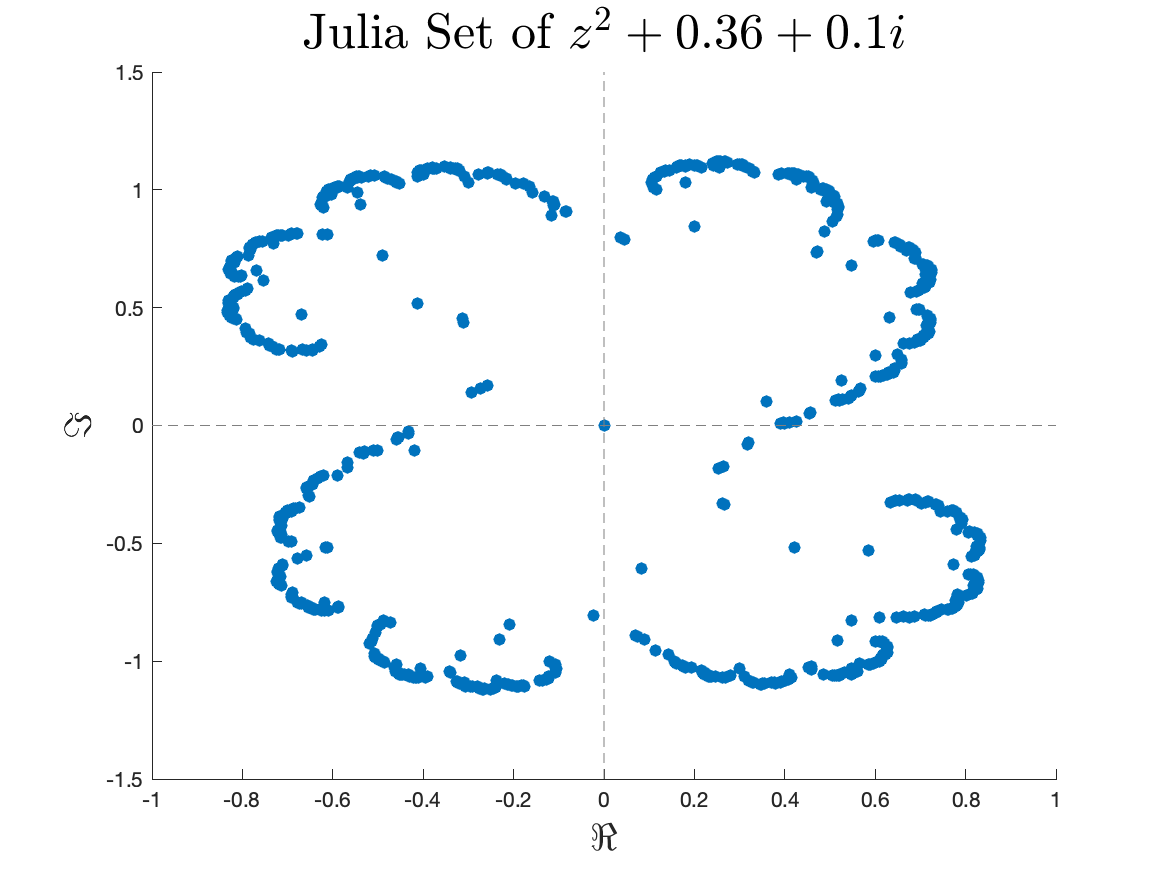
\includegraphics[width=\linewidth]{../Figures/Julia1.png}
		\caption{Julia Set of $z = 0.36 + 0.1i$}
		\label{fig:J+.36+.1i}
	\end{subfigure}
	\begin{subfigure}[b]{0.49\linewidth}
		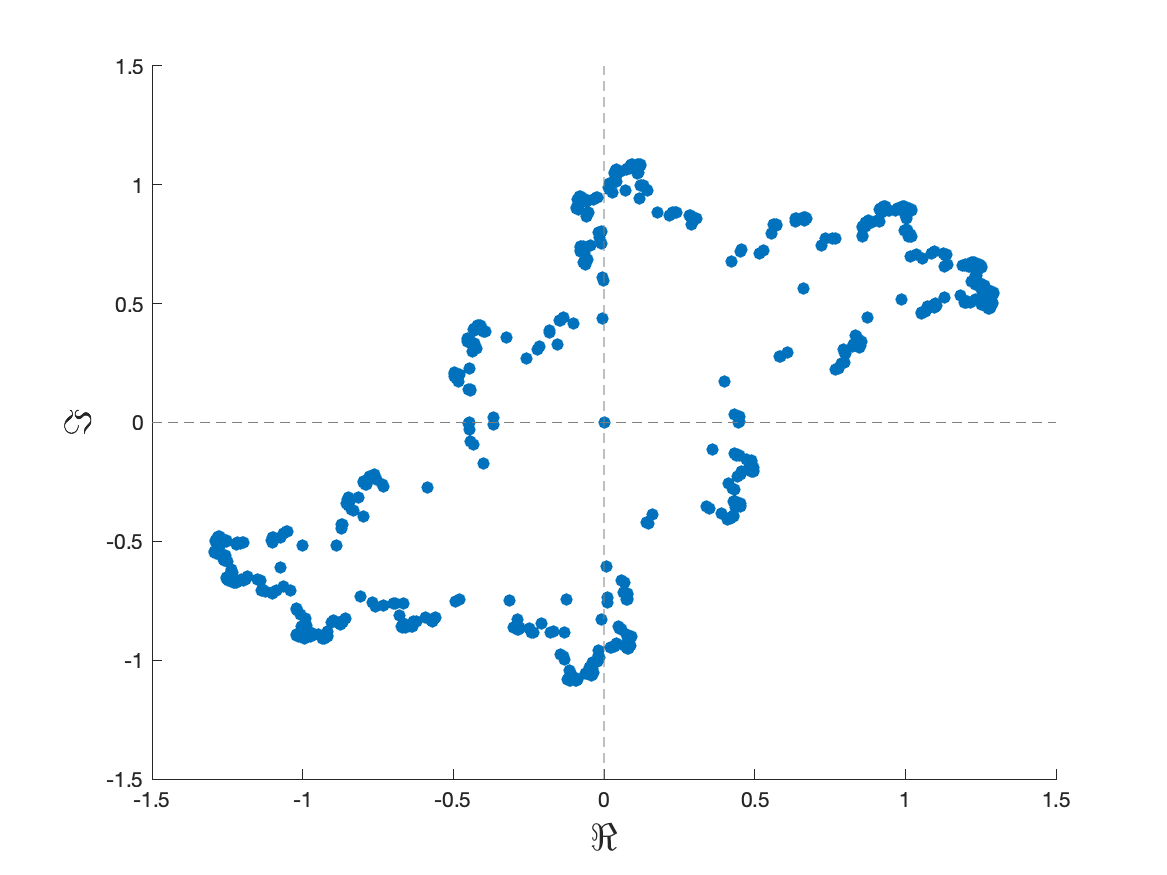
\includegraphics[width=\linewidth]{../Figures/Julia2.png}
		\caption{Julia Set of $z = -0.123 + 0.745i$}
		\label{fig:J+.123+.745i}
	\end{subfigure}
	
	\vskip\baselineskip
	
	\begin{subfigure}[b]{0.49\textwidth}
		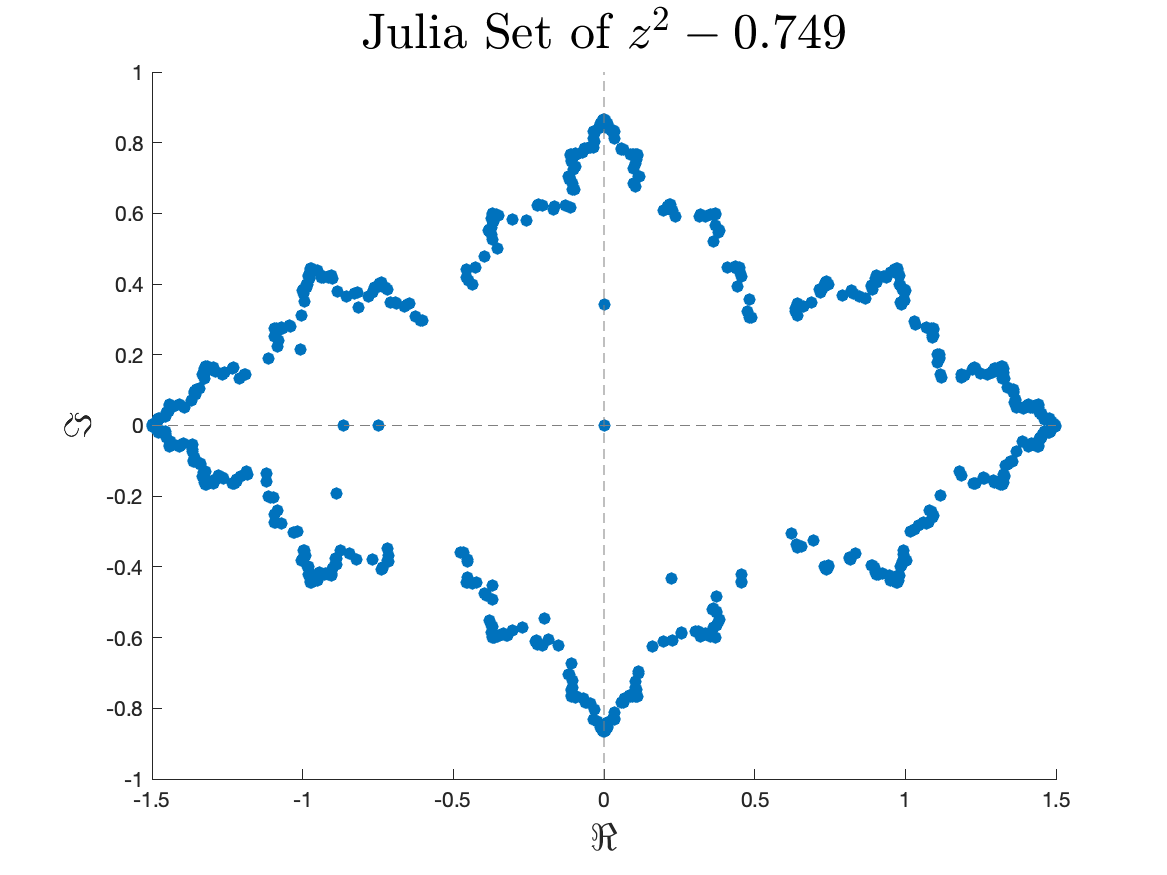
\includegraphics[width=\textwidth]{../Figures/Julia3.png}
		\caption{Julia Set of $z = - 0.749$}
		\label{fig:J-.749}
	\end{subfigure}
	\begin{subfigure}[b]{0.49\textwidth}
		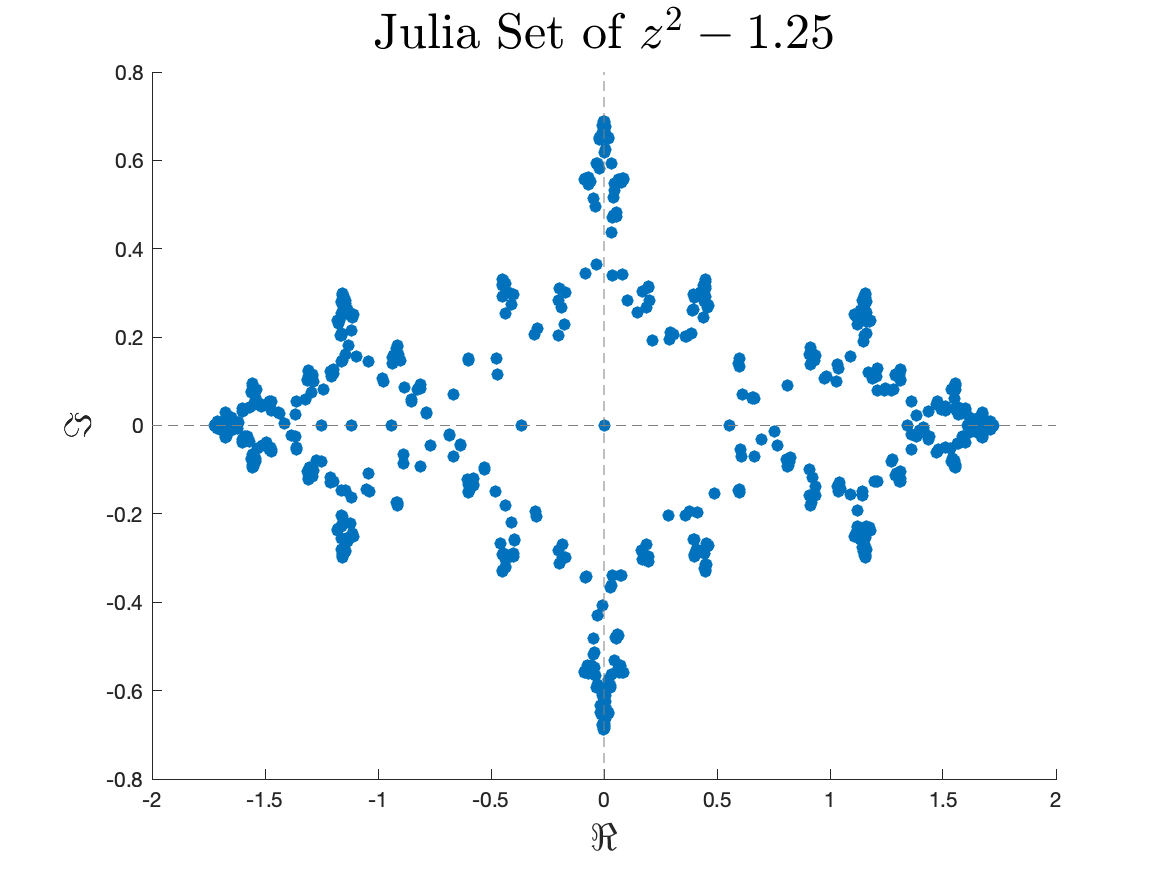
\includegraphics[width=\textwidth]{../Figures/Julia4.png}
		\caption{Julia Set of $z = -1.25$}
		\label{fig:J-1.25}
	\end{subfigure}
	\caption{Julia sets with 10,000 iterations of the inverse function}
	\label{fig:Julia}
\end{figure}

\section{Fractal Dimensions}
Fractals are shapes that don’t have integer dimensions. A line, square and cube have one, two and three dimensions respectively, while a fractal may have dimension 1.585 (Sierpinski Triangle) or 2.3 ( $\approx$ a choppy sea surface during a storm). Mathematicians measure dimension by observing the effects of scaling the length of a shape on the shape’s “mass”. For example, scaling the length of a line by $\frac{1}{2}$ creates a line $\frac{1}{2}$ the size of the original, and because $\frac{1}{2}^1=\frac{1}{2}$, a line is one dimensional. Similarly, scaling the length of a square by $\frac{1}{2}$ produces a square $\frac{1}{4}$ the size of the original, and $\frac{1}{2}^2 = \frac{1}{4}$. The same calculation can be done on a Sierpinski Triangle, although it has infinite length and zero area. Scaling a side by $\frac{1}{2}$ gives a new triangle $\frac{1}{3}$ the size of the original. $\frac{1}{2}^x = \frac{1}{3}$ invites the utilization of logarithms and gives rise to equation (1) from Bisoi and Mishra 2001. In nature, and in Julia sets for that matter, scaling factors are not so apparent and box counting coupled with least squares linear approximations through points on log-log plots must be used.

\section{Julia Set Connectivity}
A Julia set is considered connected if a point in the set can travel to another point in the set without having to leave the set. In other words, there is only one boundary that encloses all points. Julia discovered a simple criterion to determine if Julia sets are connected. He found that if the orbit of the initial point 0 is bounded, then the set is connected, otherwise it is not. Therefore, the connectivity of set under the function $\phi(z)$ can be easily found, but careful consideration must be required for the number of iterations to use. Too few iterations may not be enough to capture the diverging effect of the orbit, while too many may require an unnecessary number of computations. The algorithm in Part 5 of the code below shows how the connectivity is determined. Notice that the output never definitively states a Julia set is connected because it is not generally known if a value is truly converged when there are a finite number of iterations. It is possible a point in a set that stays bounded at the $10,000^{th}$ iteration will diverge at the $20,000^{th}$, however unlikely that may seem.

\section{Divergent Orbits}
The number of iterations it takes for a value to diverge creates interesting plots. Coloring of the orbits is according to the number of iterations that the orbits take to diverge. We used the filled Julia set functions and set the threshold of divergence to $|z| = 100$, and then used the spectrum chart to represent the number iterations by color. Points on the complex plan that took many iterations to diverge, or didn't converge at all, have a red color; while points that diverged quickly have blue color. The orbits with similar iteration number would have the similar colors. Additionally, the orbits of similar colors have similar shape and iteration numbers. Accordingly, self similarity can be found in orbits with the same color.

\begin{figure}
\centering
	\begin{subfigure}[b]{0.49\linewidth}
		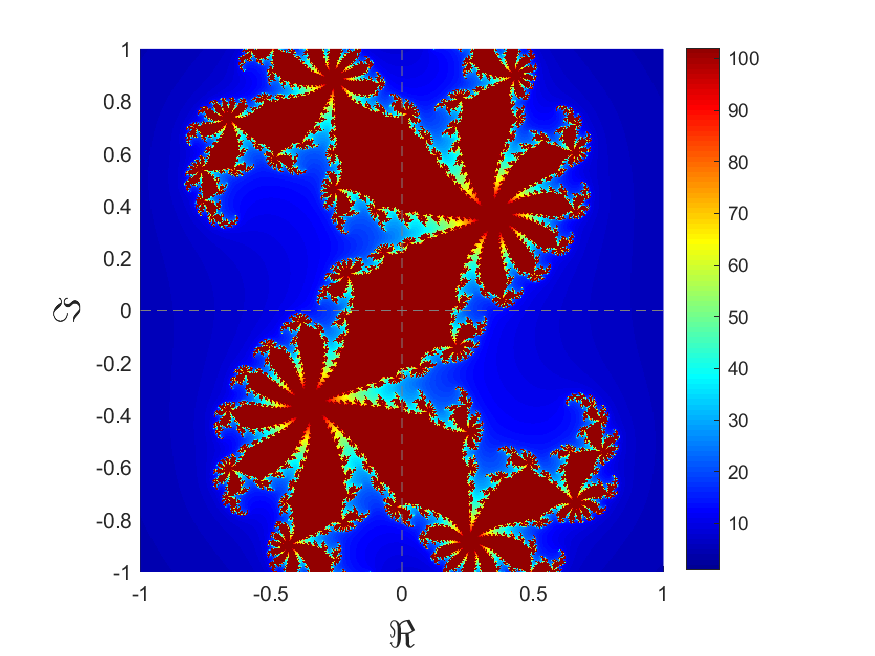
\includegraphics[width=\linewidth]{../Figures/ColoredJulia1.png}
		\caption{Julia Set of $z = 0.36 + 0.1i$}
		\label{fig:CJ+.36+.1i}
	\end{subfigure}
	\begin{subfigure}[b]{0.49\linewidth}
		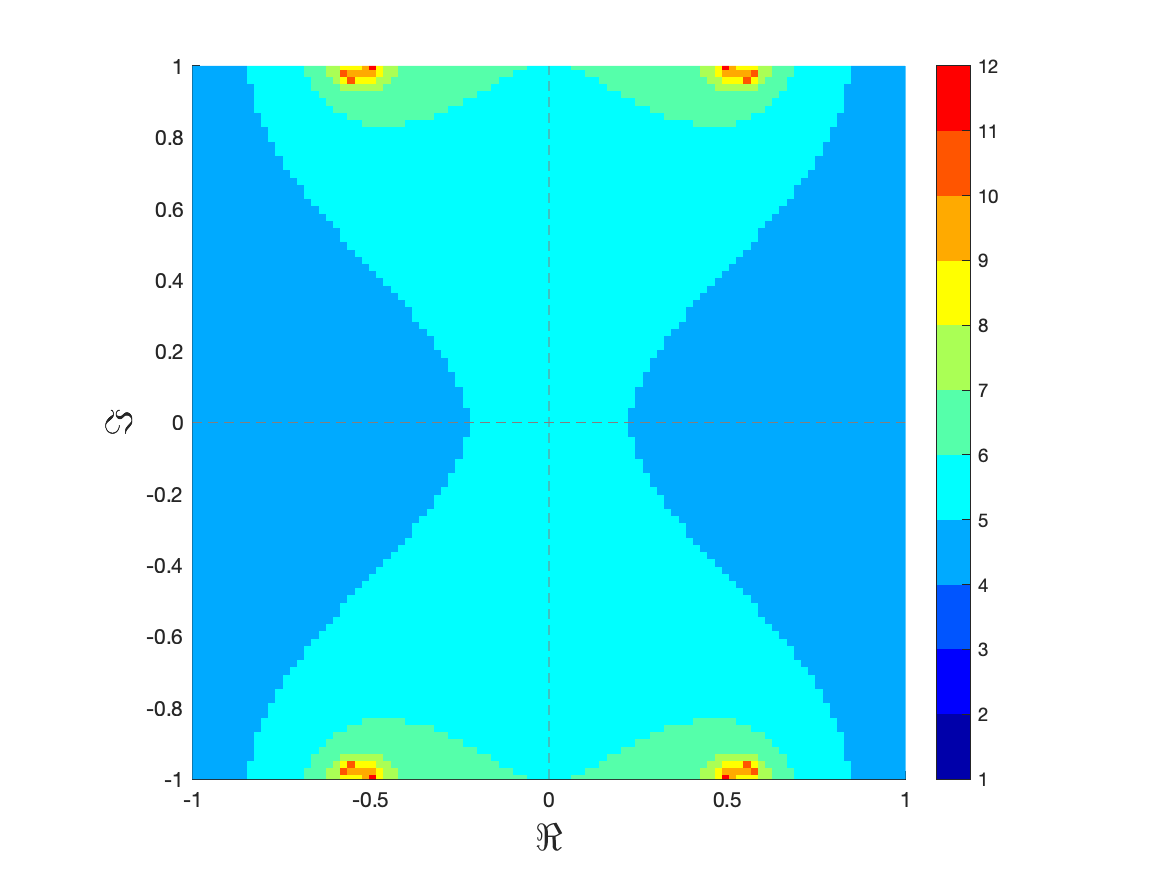
\includegraphics[width=\linewidth]{../Figures/ColoredJulia2.png}
		\caption{Julia Set of $z = -0.123 + 0.745i$}
		\label{fig:CJ+.123+.745i}
	\end{subfigure}
	
	\vskip\baselineskip
	
	\begin{subfigure}[b]{0.49\textwidth}
		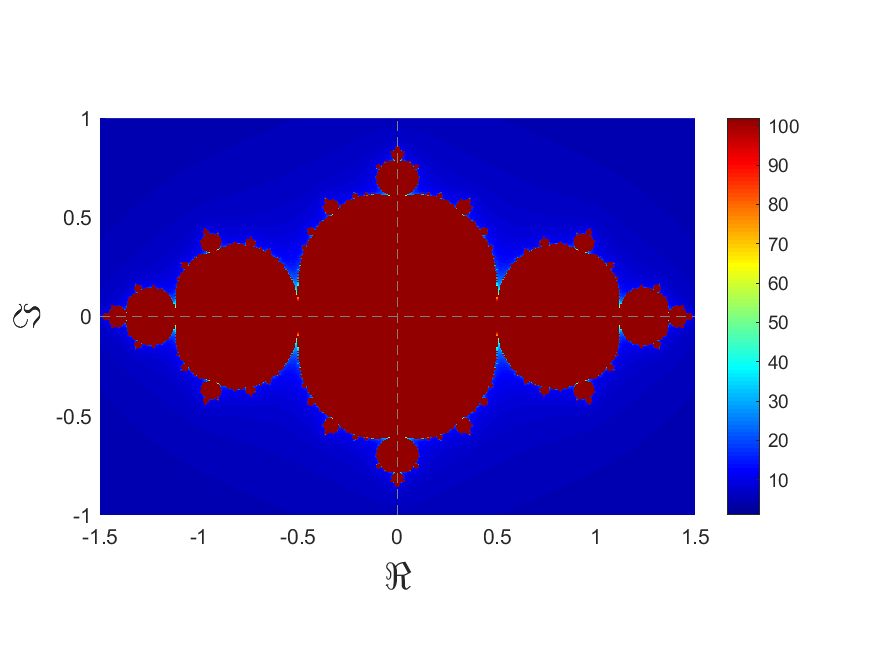
\includegraphics[width=\textwidth]{../Figures/ColoredJulia3.png}
		\caption{Julia Set of $z = - 0.749$}
		\label{fig:CJ-.749}
	\end{subfigure}
	\begin{subfigure}[b]{0.49\textwidth}
		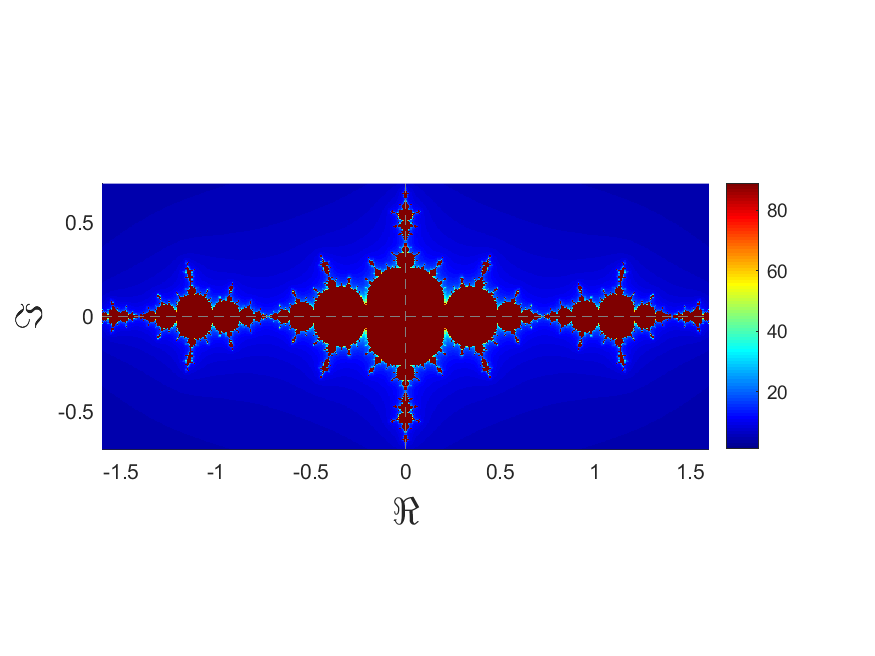
\includegraphics[width=\textwidth]{../Figures/ColoredJulia4.png}
		\caption{Julia Set of $z = -1.25$}
		\label{fig:CJ-1.25}
	\end{subfigure}
	\caption{Filled Julia sets colored based on number of iterations to diverge}
	\label{fig:CJwithC}
\end{figure}

\section{Newton's Method in Complex Plane}
Root finding can be a surprisingly difficult task. The linear case is trivial and roots of second order polynomials are solved with the quadratic equation. However, as the order increases the analytic equations to solve for the roots become more intricate and no known analytic equation exists for polynomials of orders higher than 6. Not to mention, this is just for real functions! Finding the roots of complex functions is even more difficult. Fortunately iterative methods, with the help of plots, simplify the process; although, some accuracy will be lost. The plots in figure \ref{fig:NI} are not just interesting, but also insightful. When plotting the Newton fractals and coloring the points with the number of iterations required to converge, the location of the roots become evident. For Newton's method, and any iterative method I can think of, the closer an initial guess is to a root, the less iterations are required. So the roots are found where the plots indicate the least amount of iterations are, in this case dark blue. Looking at figure \ref{fig:NI3} it appears the roots around $(1,0i), (-0.5,0.86i), (0.5,-0.86i)$. This agrees with the known values of $(1,0i), (-0.5, \frac{\sqrt{3}}{2}i), (-0.5, -\frac{\sqrt{3}}{2}i)$. The process extends to all subfigures in figure \ref{fig:NI} and to any complex function whose roots are desired.

\def\fwidth{0.49\textwidth}
\begin{figure}
\centering
	\begin{subfigure}[b]{\fwidth}
		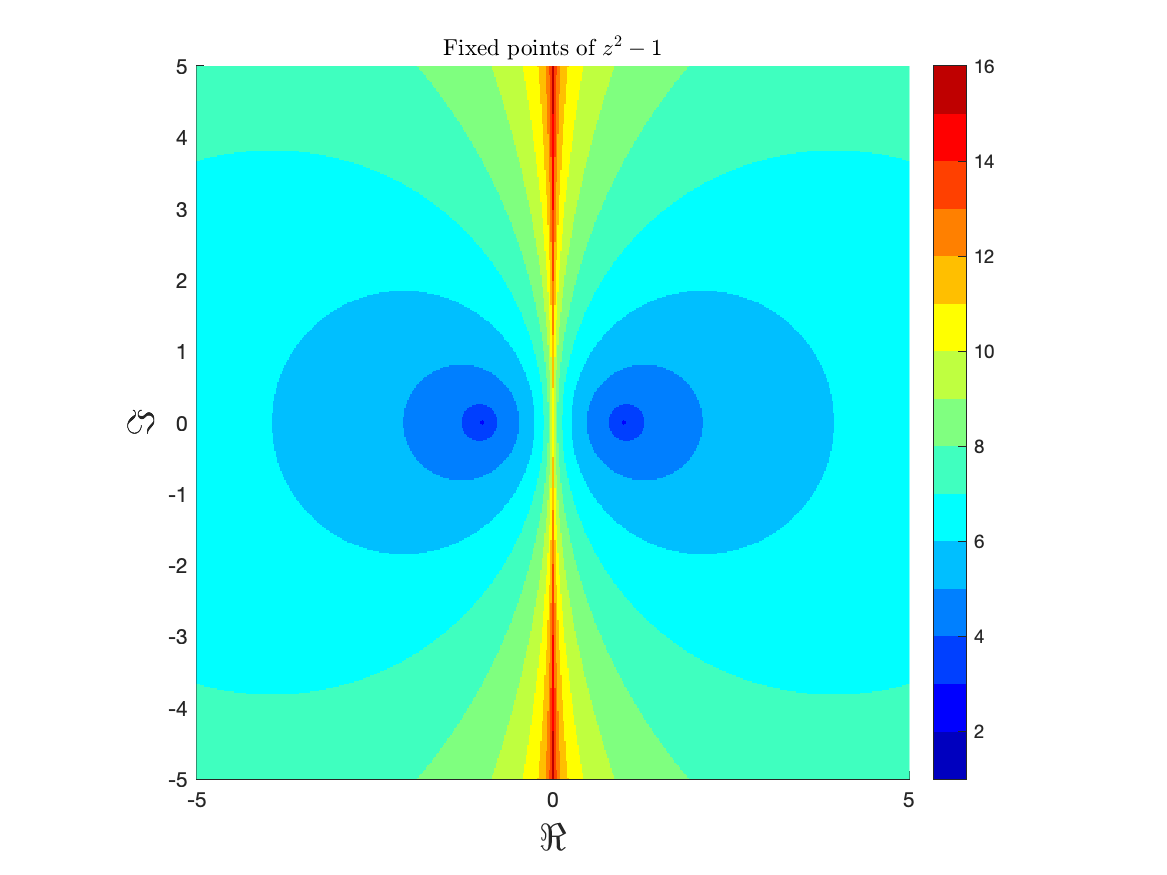
\includegraphics[width=\textwidth]{../Figures/Newton1.png}
		\caption{Iterations to roots of $z^2 - 1$}
		\label{fig:NI2}
	\end{subfigure}
	\begin{subfigure}[b]{\fwidth}
		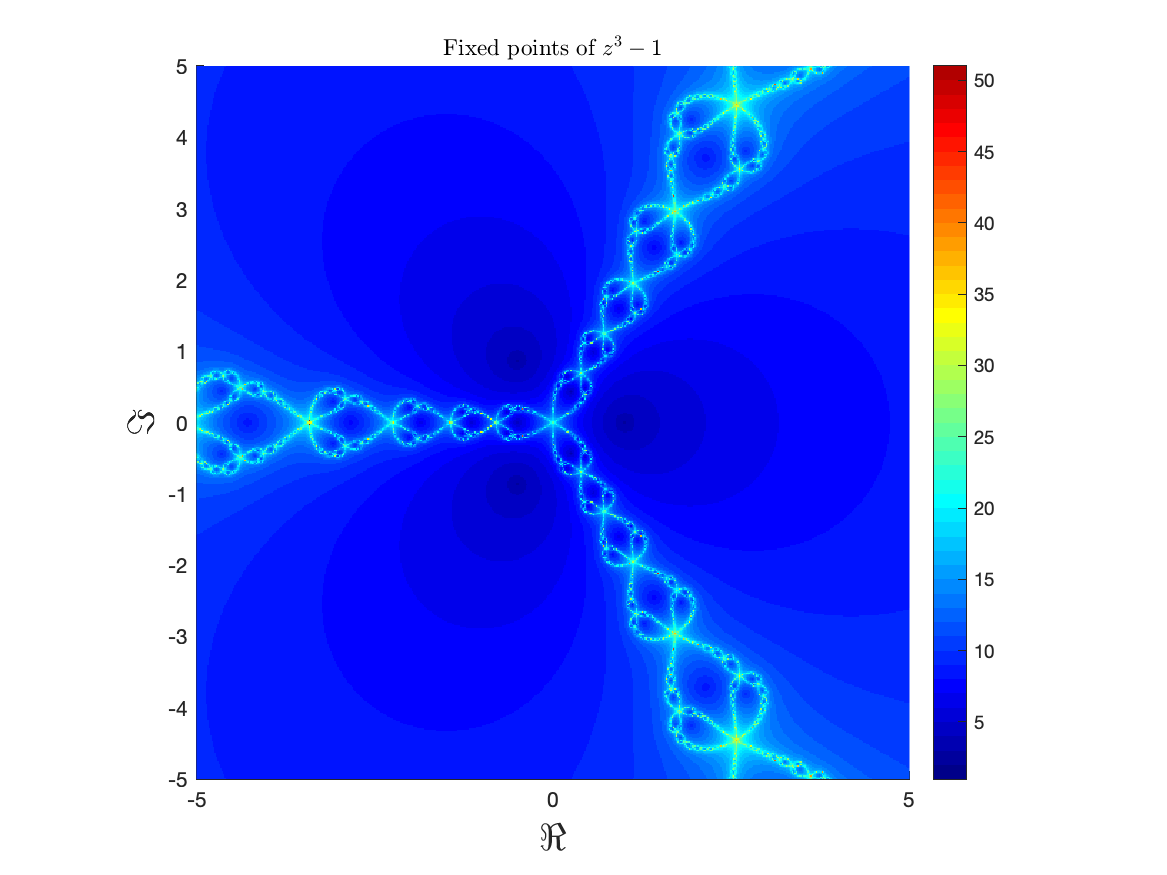
\includegraphics[width=\textwidth]{../Figures/Newton2.png}
		\caption{Iterations to roots of $z^3 - 1$}
		\label{fig:NI3}
	\end{subfigure}
	
	\vskip\baselineskip
	
	\begin{subfigure}[b]{\fwidth}
		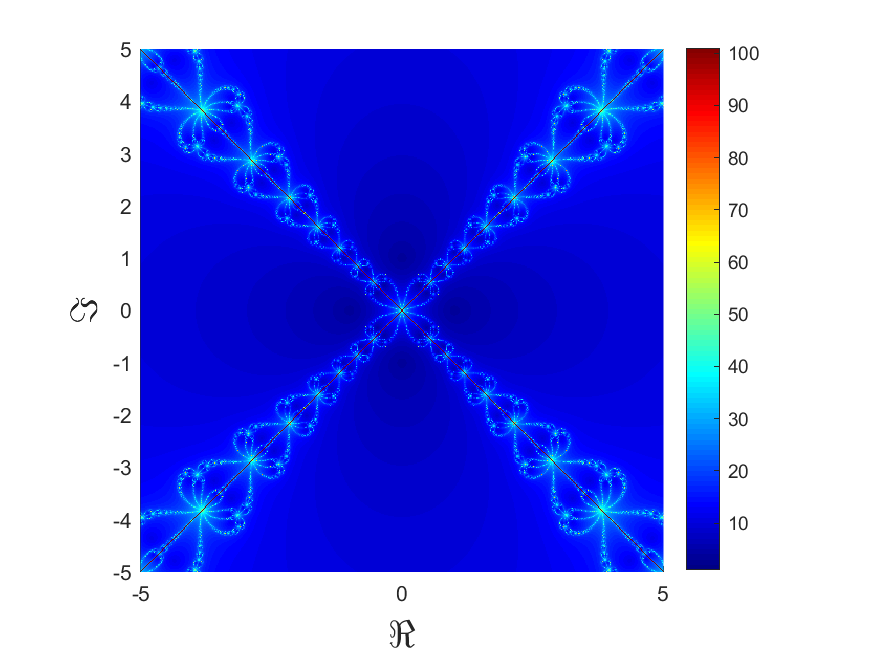
\includegraphics[width=\textwidth]{../Figures/Newton3.png}
		\caption{Iterations to roots of $z^4 - 1$}
		\label{fig:NI4}
	\end{subfigure}
	\begin{subfigure}[b]{\fwidth}
		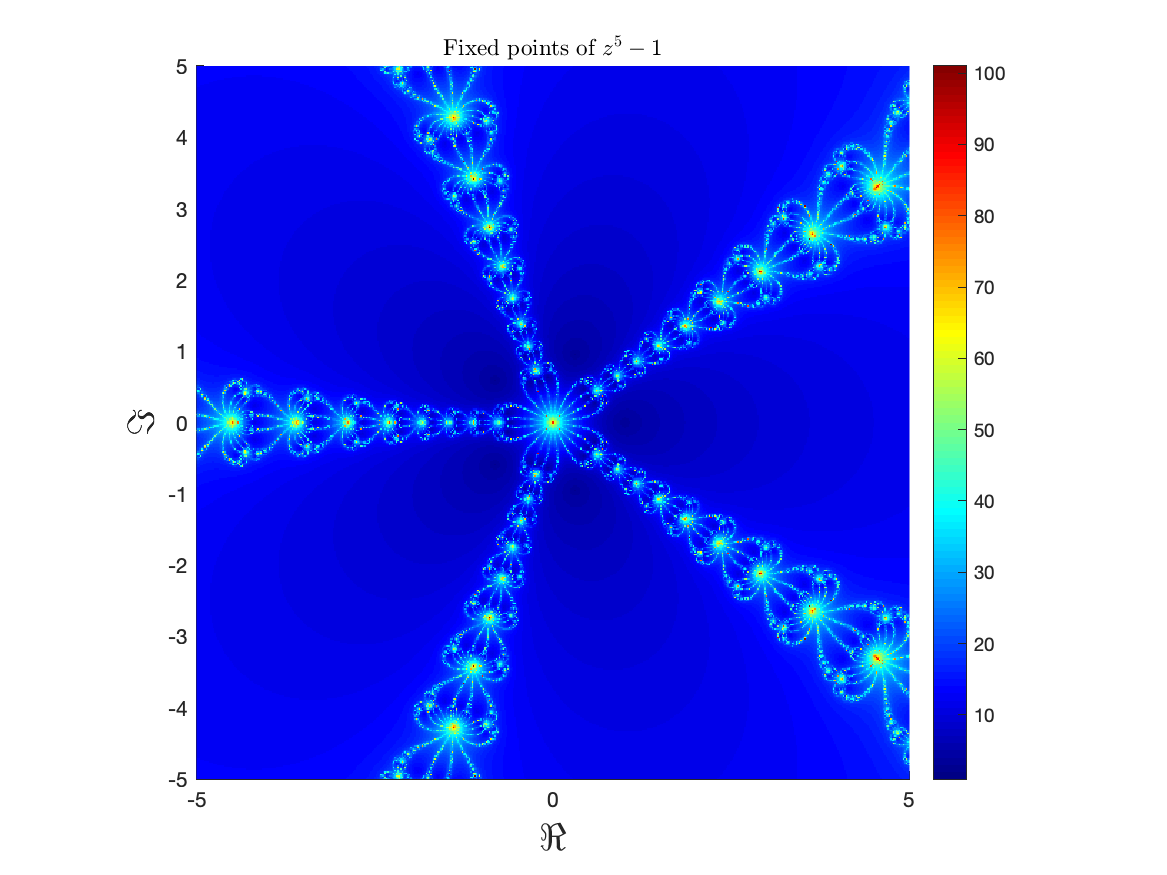
\includegraphics[width=\textwidth]{../Figures/Newton4.png}
		\caption{Iterations to roots of $z^5 - 1$}
		\label{fig:NI5}
	\end{subfigure}
	\caption{Roots of complex functions of form $z^n - 1$}
	\label{fig:NI}
\end{figure}

\section{The Mandelbrot Set}
In the Julia sets for $z_{n+1} = z^2 + c$, we fix c and cycle through $z_0$ values to create one image. Different Julia set images can be created with different values of c. In the Mandelbrot set, however, we will fix $z_0 = 0$ and cycle through all c values in the complex plane. The coloring of the image indicates the number of iterations required for the particular value to diverge. By starting with an initial point at the origin and searching through different constants in the complex plane the Mandelbrot set must be all values of c such that the Julia sets are connected, since bounded orbits of 0 form connected Julia sets.

\begin{figure}
	\centering
	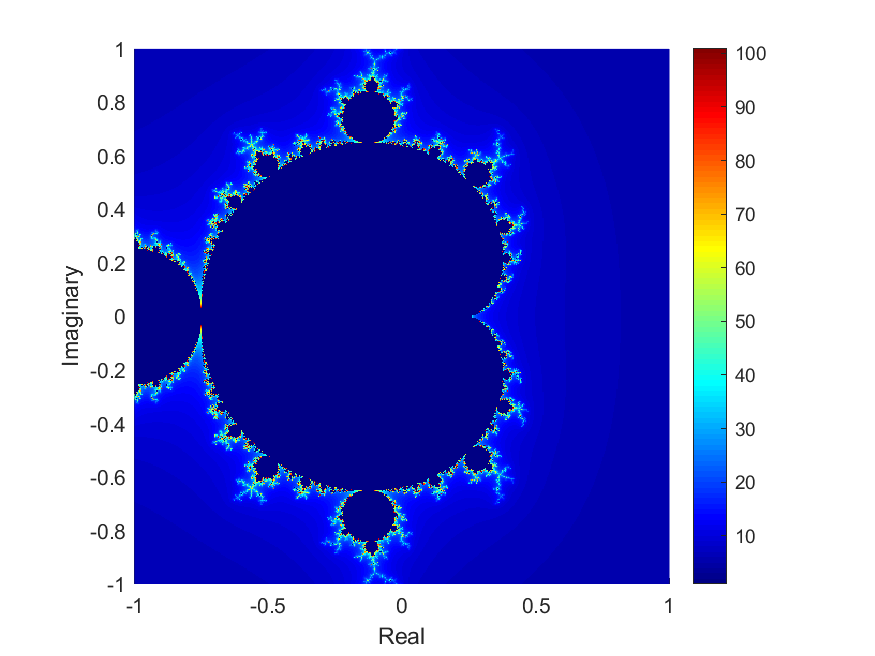
\includegraphics[width=3.5in]{../Figures/Mandelbrot.png}
	\caption{Mandelbrot set showing which constants for a connected Julia Set under $\psi = z^2 + c$}
	\label{fig:Mandelbrot}
\end{figure}

\section{Conclusion}
Fractals are interesting shapes that come about when finding the orbits of complex functions. Due to the iterative nature of orbits, visually representing them was a lengthy process. However, with computers, fractals can be easily visualized. One can switch the function under which the orbit is to be calculated by changing a few values. Previously, this would have required manually recalculating the orbit of each point. Fractals, which gets its name from fractional dimensions, are more than just interesting shapes. Fractals can represent important values for problem solving. Take Newton's iterations for example, the roots of an equation can be found by observing which values in the domain converge to a root the fastest. 

\newpage

\section{Appendix}

\subsection{Code}
\lstinputlisting[breaklines=true]{../Code/Project1.m}

\subsection{Group Work}
The group met on several occasions to discuss division of work and how to collaborate. We initially used a divide and conquer method, but began collaborating as the problems were challenging and we needed the skills and knowledge of the whole group. Nikos and Caitlin collaborated on the first two problems, while Shuai and Nikos worked on the coloring of Julia sets. Shuai and Nikos also worked on using polar coordinates for the Julia set boundary, but we resulted in using cartesian coordinates for its simpler implementation which still gave good results. Caitlin did the background reading and code for calculating the fractal dimension. For the first part, generating the unit disk, Nikos created a function for calculating the Julia set, which in turn could be used for many of the other parts of the project. So the same function was repurposed for part ii, iv, and vi. As the Mandelbrot set and calculating the connectivity of Julia set were similar to the other Julia set questions, Nikos created the code for that as well. Nikos did background reading and the algorithm implementation for part vii, Newton's Method in the complex plane. As for the report, everyone contributed to the sections they worked on. 

\end{document}
